% -*- compile-command: "make HOCKING-peak-penalty-slides.pdf" -*-
\documentclass{beamer}
\usepackage{tikz}
\usepackage[all]{xy}
\usepackage{amsmath,amssymb}
\usepackage{hyperref}
\usepackage{graphicx}

\DeclareMathOperator*{\argmin}{arg\,min}
\DeclareMathOperator*{\Lik}{Lik}
\DeclareMathOperator*{\Peaks}{Peaks}
\DeclareMathOperator*{\Segments}{Segments}
\DeclareMathOperator*{\argmax}{arg\,max}
\DeclareMathOperator*{\maximize}{maximize}
\DeclareMathOperator*{\minimize}{minimize}
\newcommand{\sign}{\operatorname{sign}}
\newcommand{\RR}{\mathbb R}
\newcommand{\ZZ}{\mathbb Z}
\newcommand{\NN}{\mathbb N}

% Set transparency of non-highlighted sections in the table of
% contents slide.
\setbeamertemplate{section in toc shaded}[default][100]
\AtBeginSection[]
{
  \setbeamercolor{section in toc}{fg=red} 
  \setbeamercolor{section in toc shaded}{fg=black} 
  \begin{frame}
    \tableofcontents[currentsection]
  \end{frame}
}

\begin{document}

\title{A qsub pipeline for 
  supervised ChIP-seq peak detection} 

\author{
  Toby Dylan Hocking\\
  toby.hocking@mail.mcgill.ca\\
  joint work with Guillem Rigaill and Guillaume Bourque}

\date{2 April 2015}

\maketitle

\section{ChIP-seq data and previous work on unsupervised peak
  detection}


\begin{frame}
  \frametitle{Chromatin immunoprecipitation sequencing (ChIP-seq)}
  Analysis of DNA-protein interactions.

  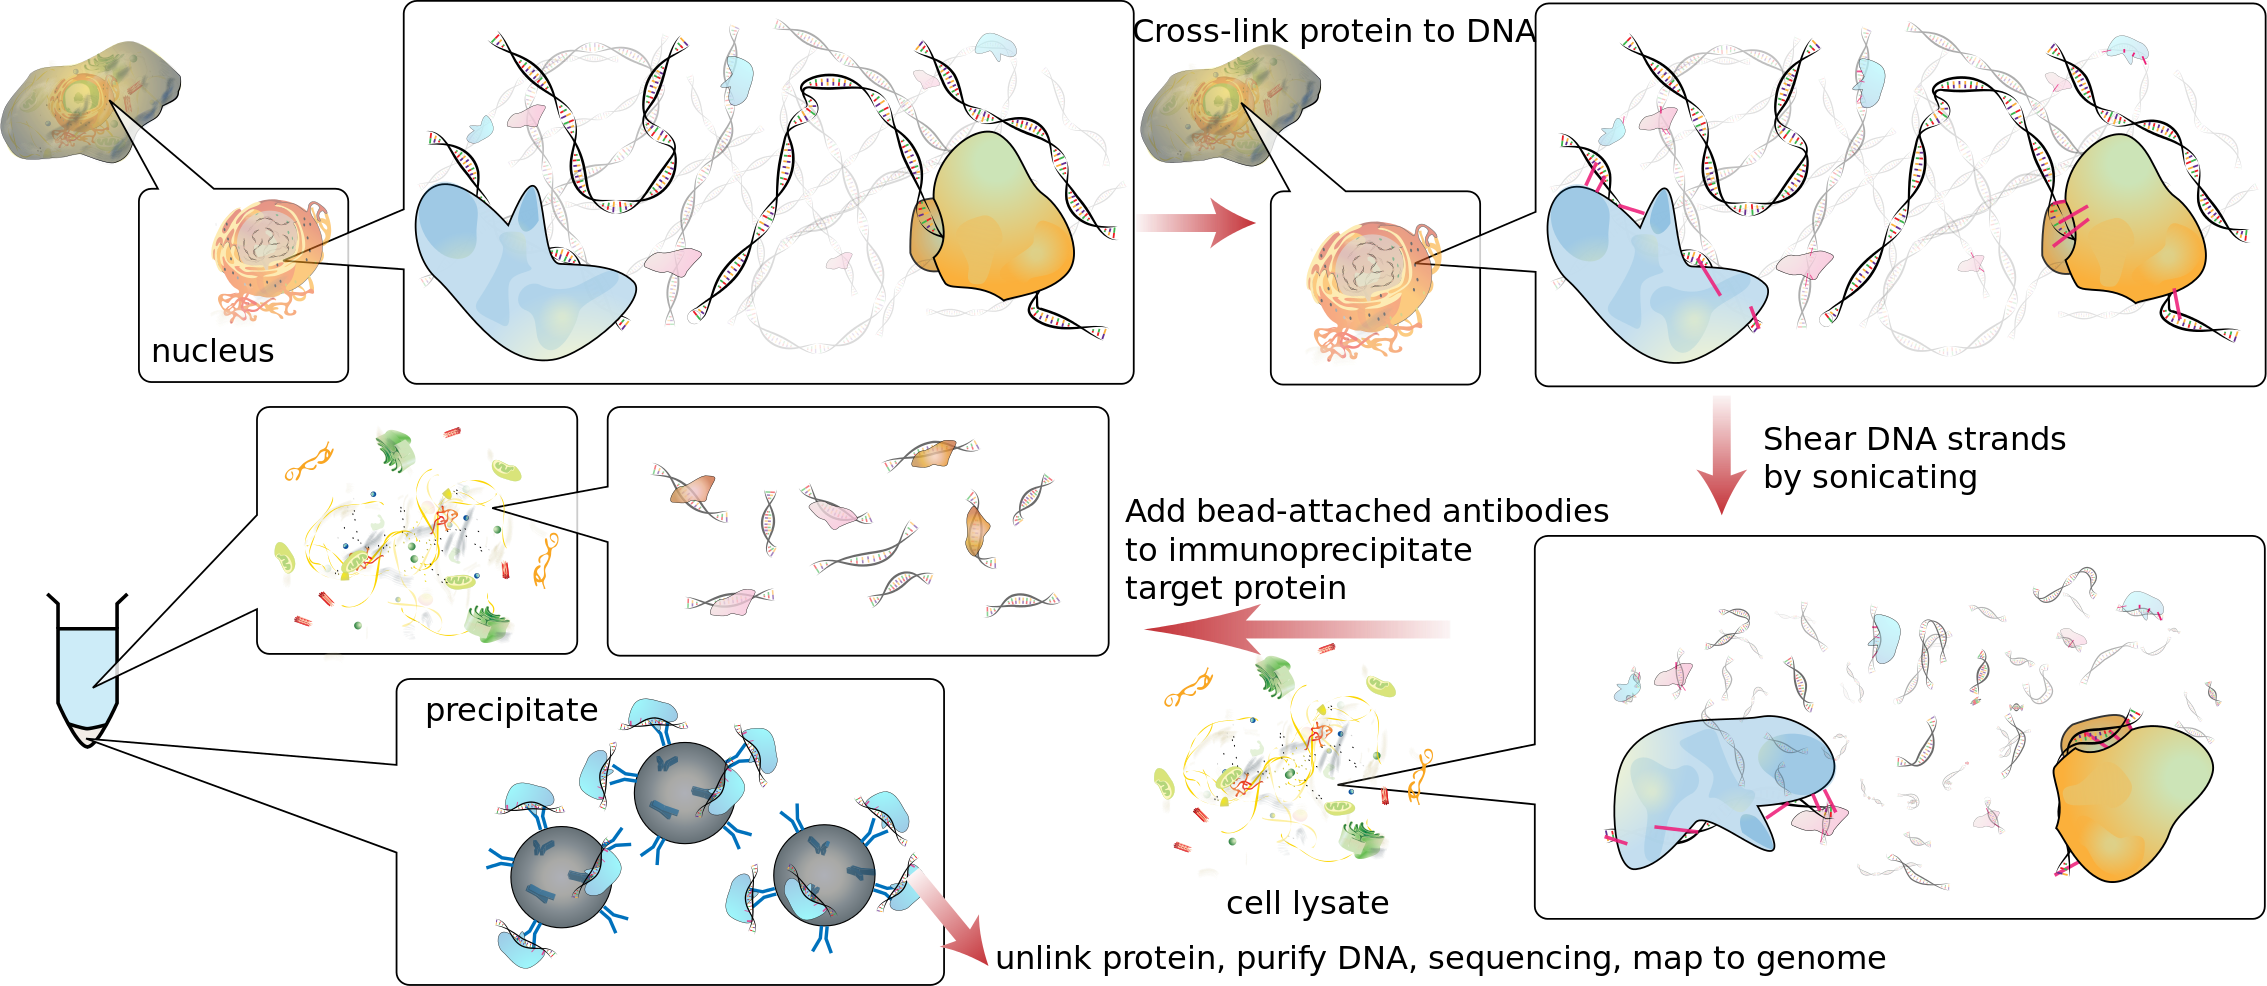
\includegraphics[width=\textwidth]{Chromatin_immunoprecipitation_sequencing_wide.png}

  Source: ``ChIP-sequencing,'' Wikipedia.
\end{frame}

\begin{frame}
  \frametitle{Data downloaded from Epigenomes Portal}
  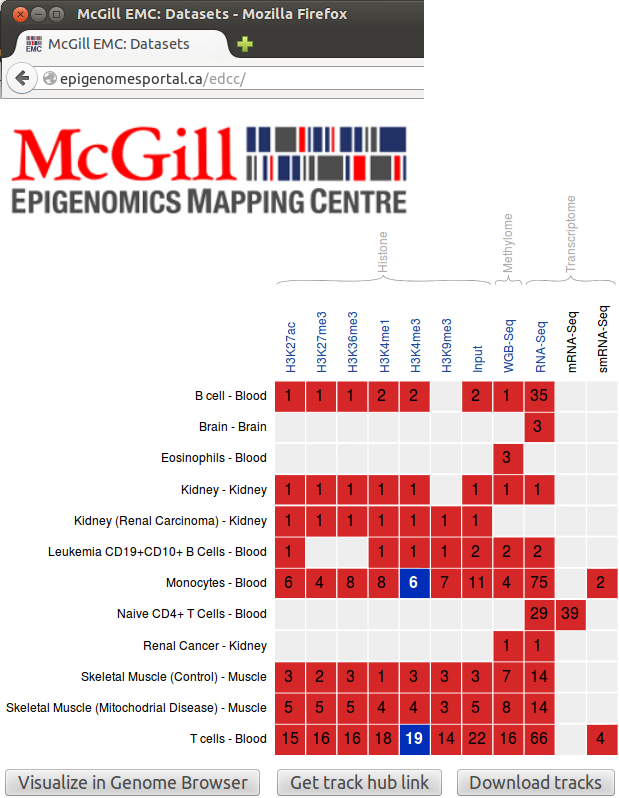
\includegraphics[width=2.5in]{screenshot-samples}
\end{frame}

\begin{frame}
  \frametitle{Goal: find peaks in each of several samples}
  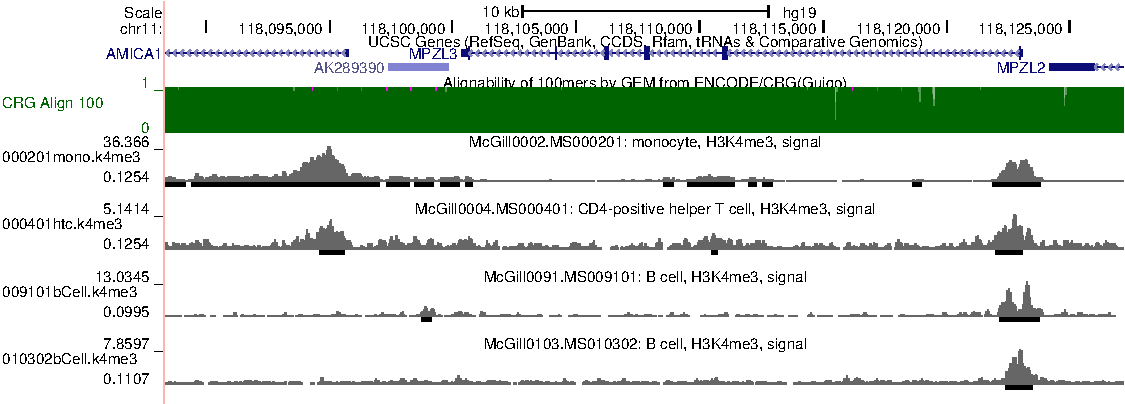
\includegraphics[width=\textwidth]{screenshot-ucsc-edited}
\end{frame}

\begin{frame}
  \frametitle{Existing unsupervised peak detection algorithms}
  \begin{itemize}
  \item Model-based analysis of ChIP-Seq (MACS), Zhang et al, 2008.
  \item SICER, Zang et al, 2009.
  \item HOMER findPeaks, Heinz et al, 2010.
  \item RSEG, Song and Smith, 2011.
  \item Histone modifications in cancer (HMCan), Ashoor et al, 2013.
  \item ... dozens of others.
  \end{itemize}
  Two big questions: how to choose the best...
  \begin{itemize}
  \item ...algorithm?
  \item ...parameters?
  \end{itemize}
\end{frame}

\begin{frame}[fragile]
  \frametitle{Problem: how to choose model parameters?}
\scriptsize
19 parameters for Model-based analysis of ChIP-Seq (MACS), Zhang et al, 2008.
\begin{verbatim}
  [-g GSIZE]
  [-s TSIZE] [--bw BW] [-m MFOLD MFOLD] [--fix-bimodal]
  [--nomodel] [--extsize EXTSIZE | --shiftsize SHIFTSIZE]
  [-q QVALUE | -p PVALUE | -F FOLDENRICHMENT] [--to-large]
  [--down-sample] [--seed SEED] [--nolambda]
  [--slocal SMALLLOCAL] [--llocal LARGELOCAL]
  [--shift-control] [--half-ext] [--broad]
  [--broad-cutoff BROADCUTOFF] [--call-summits]
\end{verbatim}
10 parameters for Histone modifications in cancer (HMCan),
Ashoor et al, 2013.
\begin{verbatim}
minLength 145
medLength 150
maxLength 155
smallBinLength 50
largeBinLength 100000
pvalueThreshold 0.01
mergeDistance 200
iterationThreshold 5
finalThreshold 0
maxIter 20
\end{verbatim}
\end{frame}

\begin{frame}
  \frametitle{Summary of unsupervised peak detectors}
  \begin{displaymath}
  \xymatrix{
    \texttt{coverage.bedGraph}
    \ar [dr] 
    & \text{ }
    & \text{Parameters} 
    \ar [dl]
    \\
    & \texttt{peaks.bed}
  }
  \end{displaymath}
  
\end{frame}

\section{Supervised peak detection using annotated region labels}

\begin{frame}
  \frametitle{Previous work in computer vision: look and add labels
    to...}
  \begin{tabular}{ccc}
    Photos & Cell images & Copy number profiles \\
    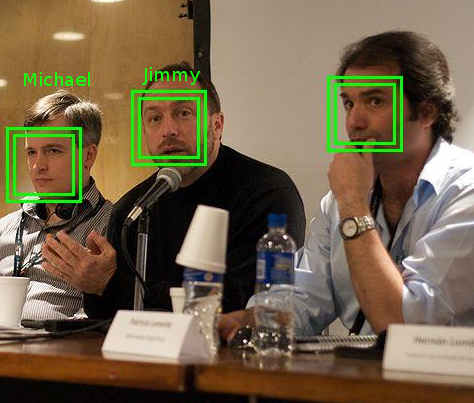
\includegraphics[width=1.3in]{faces} &
    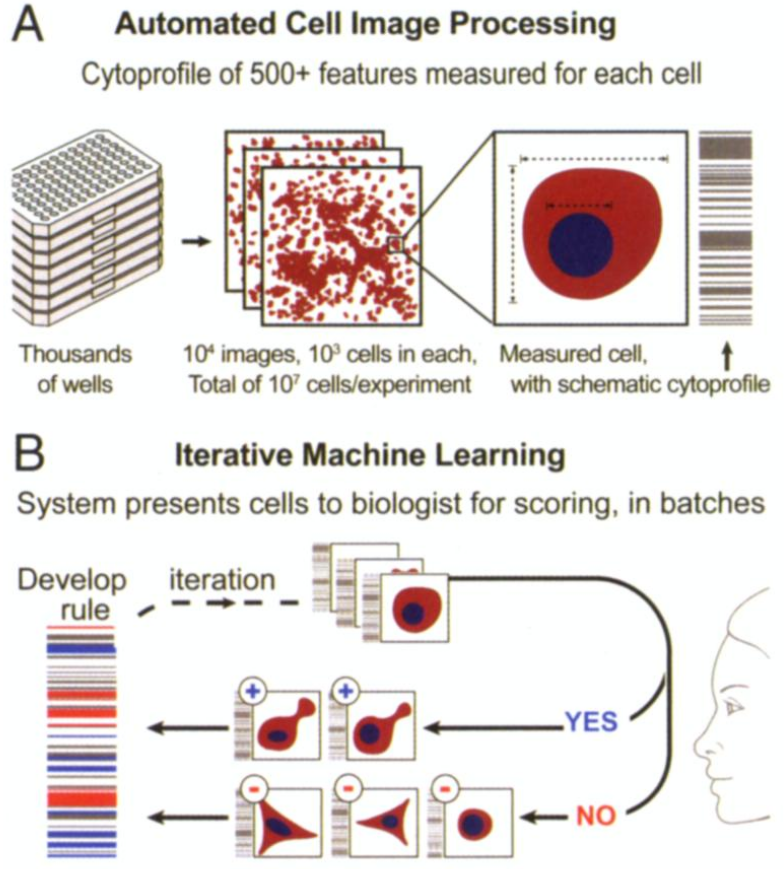
\includegraphics[width=1.3in]{cellprofiler} &
    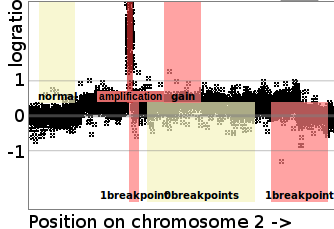
\includegraphics[width=1.5in]{regions-axes}\\
    Labels: names & phenotypes & alterations \\ \\
    CVPR 2013 & CellProfiler & SegAnnDB \\
    246 papers & 873 citations & H, \emph{et. al.} 2014. \\
     &
  \end{tabular}
  Sources: \url{http://en.wikipedia.org/wiki/Face_detection}\\
  Jones et al PNAS 2009. Scoring diverse cellular morphologies in
  image-based screens with iterative feedback and machine learning.
\end{frame}

\begin{frame}
  \frametitle{Peak detector accuracy can be quantified using manually
    annotated region labels}
  
  \includegraphics[width=1.1\textwidth]{figure-good-bad}

  \begin{itemize}
  \item Good peaks have 0 incorrect regions.
  \item Bad peaks have 7 incorrect regions.
  \item Goal: minimize number of incorrect regions.
  \end{itemize}

\end{frame}

\begin{frame}
  \frametitle{Summary of supervised peak detection}
  \begin{displaymath}
  \xymatrix{
    & & \texttt{labels.bed} \ar [d]
    \\
    \texttt{coverage.bedGraph}
    \ar [dr] 
    & \text{ }
    & \text{Parameters} 
    \ar [dl]
    \\
    & \texttt{peaks.bed}
  }
  \end{displaymath}
  
\end{frame}


\begin{frame}
  \frametitle{PeakSeg constrained maximum likelihood model}
  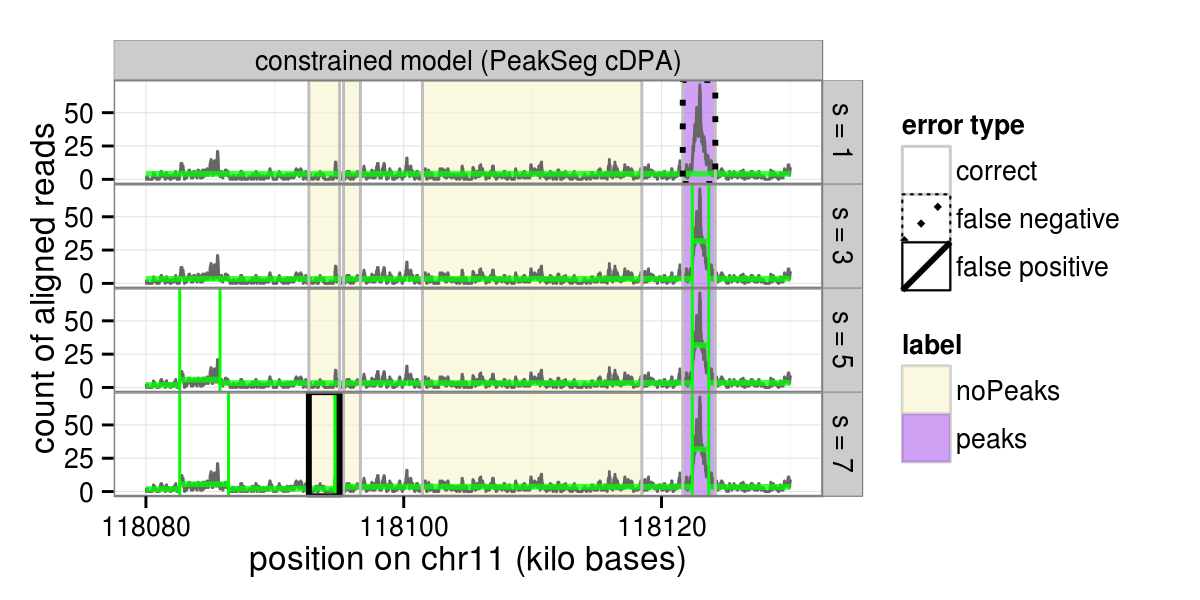
\includegraphics[width=\textwidth]{figure-Segmentor-PeakSeg-constrained-regions}

  State-of-the-art peak detection (Hocking et al, ICML2015), but
  constrained Dynamic Programming Algorithm = cDPA has
  $O(s_{\text{max}} d^2)$ time complexity:
  \begin{itemize}
  \item $s_{\text{max}}$ = maximum number of segments/peaks,
  \item $d$ = data points to segment.
  \end{itemize}
\end{frame}

\begin{frame}
  \frametitle{Timings on benchmark data sets}
  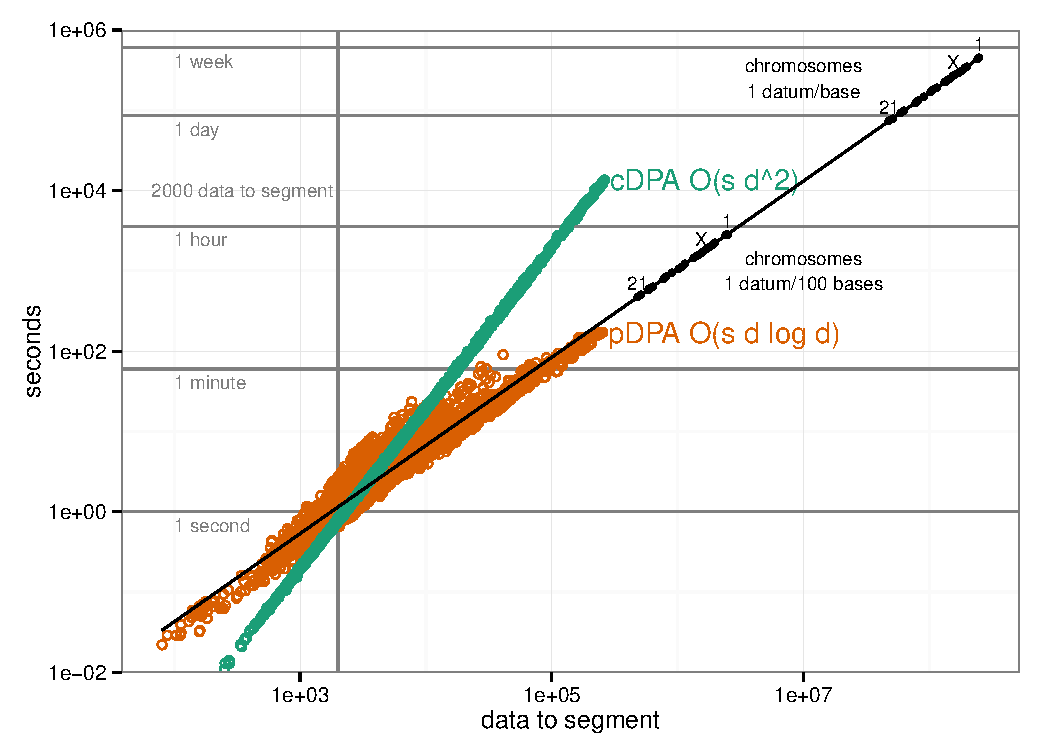
\includegraphics[width=\textwidth]{figure-cDPA-pDPA-timings}

  How to use cDPA on whole genome?
\end{frame}

\begin{frame}
  \frametitle{Summary of proposed PeakSeg model}
  Parallelizable on samples, genomic regions:
  \begin{itemize}
  \item Inputs: a ChIP-seq coverage profile $\mathbf y\in\ZZ_+^d$,\\
    maximum number of segments $s_{\text{max}}$.
  \item Proposed method: cDPA = constrained 
    %pruned 
    dynamic programming
    algorithm,
    %$O(p_{\text{max}} d \log d)$ time complexity.
    $O(s_{\text{max}} d^2)$ time complexity.
  \item Outputs: constrained maximum likelihood segmentations
    $\mathbf{\tilde m}^1(\mathbf y), 
    \dots, 
    \mathbf{\tilde m}^{s_\text{max}}(\mathbf y)$ 
    (peaks are 2nd, 4th, ... segments).
  \end{itemize}
  How to choose the optimal number of segments/peaks?\\
  Manually annotated regions + supervised penalty function learning.\\
  %(next slide).
  G Rigaill, TD Hocking, \emph{et al.} Learning Sparse Penalties for
  Change Point Detection using Max Margin Interval Regression, ICML
  2013.
\end{frame}

\section{A qsub pipeline for supervised peak detection}


\section{Results on the McGill benchmark data set, conclusions}

\begin{frame}
  \frametitle{Benchmark: 7 annotated region data sets}
  \url{http://cbio.ensmp.fr/~thocking/chip-seq-chunk-db/}
  \begin{itemize}
  \item 4 annotators (AM, TDH, PGP, XJ).
  \item 8 cell types.
  \item 37 annotated H3K4me3 profiles (sharp peaks).
  \item 29 annotated H3K36me3 profiles (broadly enriched domains).
  \item 12,826 annotated regions in total.
  %\item 2752 separate segmentation problems.
  \end{itemize}
  % Used the cDPA on the annotated data.
  % \begin{itemize}
  % \item cDPA computed models with $0, \dots, 9$ peaks\\
  %   (for 99.5\% of problems).
  % \item For the biggest problem, cDPA took 3 hours.\\
  %   ($d=88,509$ data points, 3.5 megabases)
  % \item macs takes about 90 minutes for one whole genome.
  % \end{itemize}
\end{frame}

\begin{frame}
  \frametitle{Best results on H3K4me3 data}
  \includegraphics[width=\textwidth]{figure-dp-peaks-train-1}
\end{frame}

\begin{frame}
  \frametitle{Best results on H3K36me3 data}
  \includegraphics[width=\textwidth]{figure-dp-peaks-train-2}
\end{frame}

\begin{frame}
  \frametitle{hmcan.broad better for H3K36me3, macs better for
    H3K4me3}

  \includegraphics[width=\textwidth]{figure-dp-peaks-regression-dots-unsupervised}
  
  Six train/test splits (open circles) and mean (shaded circle).
\end{frame}

\begin{frame}
  \frametitle{Training 1 parameter with grid search reduces test error}

  ...except for macs, good defaults for 3/4 H3K4me3 data sets.

  \includegraphics[width=\textwidth]{figure-dp-peaks-regression-dots-grid}

  Six train/test splits (open circles) and mean (shaded circle).
\end{frame}

\begin{frame}
  \frametitle{Supervised genome-wide PeakSeg method works for both
    data types}

  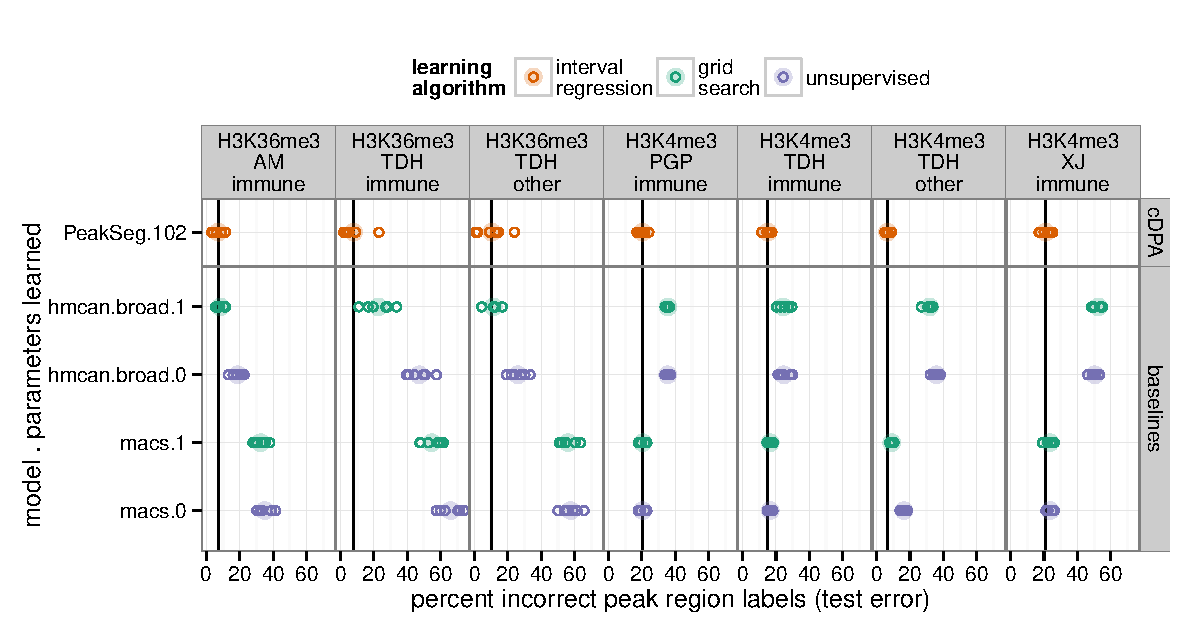
\includegraphics[width=\textwidth]{figure-dp-peaks-regression-dots}

  Six train/test splits (open circles) and mean (shaded circle).
\end{frame}

\begin{frame}
  \frametitle{Conclusions and future work}
  PeakSeg: \textbf{Peak} detection via constrained optimal
  \textbf{Seg}mentation.
  \begin{itemize}
  \item First peak detector with efficient multi-parameter supervised
    learning algorithm.
  \item State-of-the-art peak detection for both H3K4me3 and H3K36me3
    profiles.
  \end{itemize}
  Future work:
  \begin{itemize}
  \item Detecting the same peaks across several profiles?
  \item Faster algorithm via constrained version of
    \begin{tabular}{rllll}
      Time & Models & Algorithm & Author 
      % & Reference 
      \\
      \hline
      $O( s_{\text{max}} d\log d)$ & $s_{\text{max}}$ &
      pDPA & Rigaill 
      % & arXiv:1004.0887 
      \\
      $O(d\log d)$ & 1 & FPOP & Maistone et al. % & arXiv:1409.1842 
    \end{tabular}
    \\
    $d$ = data points to segment, $s_{\text{max}}$ = max segments.
  \end{itemize}
\end{frame}

\begin{frame}
  \frametitle{Thanks for your attention!}
  Write me at \alert{\texttt{toby.hocking@mail.mcgill.ca}} to collaborate!

  \vskip 1cm

  Source code for slides, figures, paper online!\\
  \small
  \url{https://github.com/tdhock/PeakSeg-paper}
  \vskip 1cm

  Supplementary slides appear after this one.

\end{frame}

\begin{frame}
  \frametitle{Two annotators provide consistent labels, but different
    precision}
  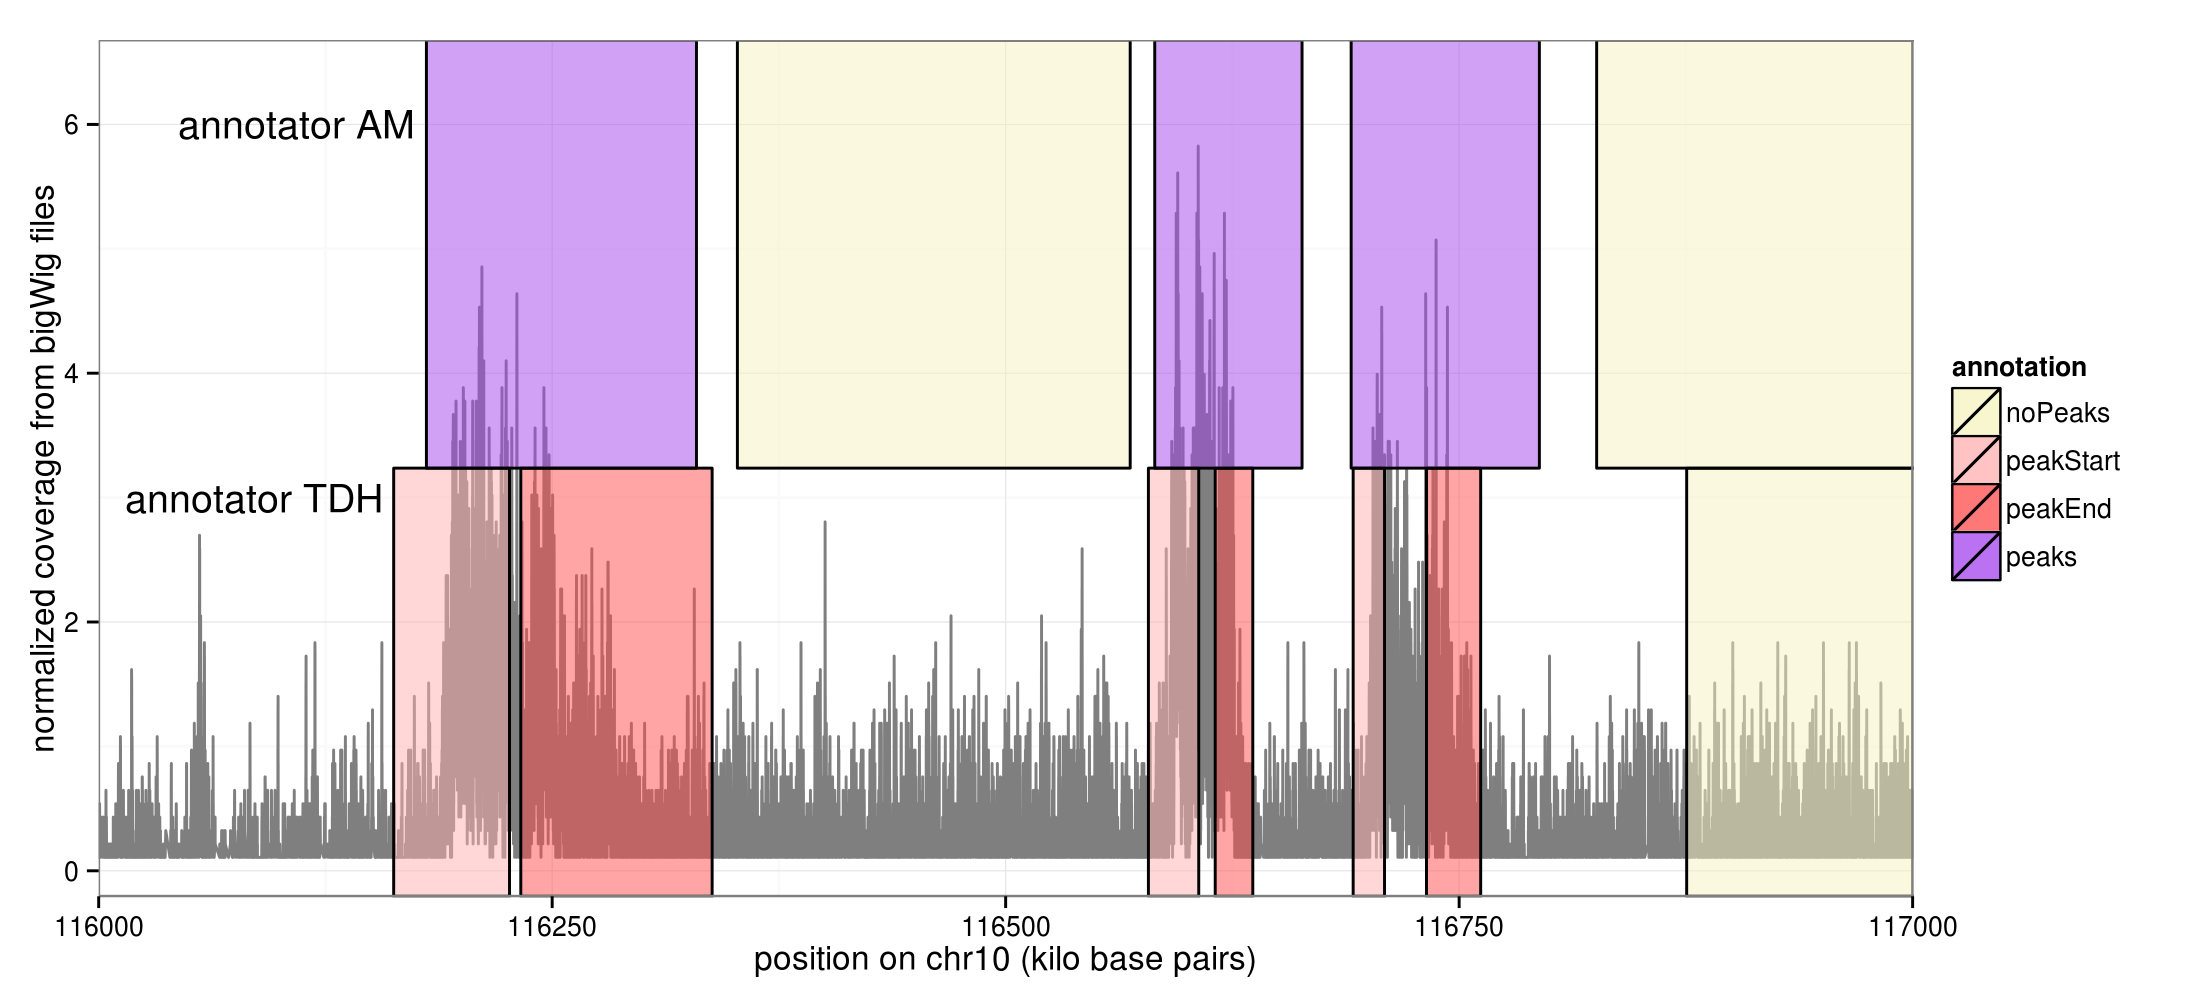
\includegraphics[width=1.1\textwidth]{figure-several-annotators}

  \begin{itemize}
  \item TDH peakStart/peakEnd more precise than AM peaks.
  \item AM noPeaks more precise than TDH no label.
  \end{itemize}
\end{frame}


\begin{frame}
  \frametitle{Maximum likelihood segmentations}
  For a coverage profile $\mathbf y\in\ZZ_+^d$,
  find the mean vector $\mathbf{\hat m}^s(\mathbf y)\in\RR^d$ with
  maximum Poisson likelihood, given $s$ segments ($s-1$ change-points).

  \includegraphics[width=\textwidth]{figure-Segmentor-PeakSeg-unconstrained}

  Computed via Segmentor3IsBack R package (Cleynen et al. 2014)

\end{frame}

\begin{frame}
  \frametitle{Previous work: maximum likelihood segmentation}
  \begin{itemize}
  \item   Let $\mathbf y = 
\left[
  \begin{array}{ccc}
    y_1 & \cdots & y_d
  \end{array}
\right]
\in\ZZ_+^d$ be the aligned read counts for one sample
  and one genomic region.
%\item For example the biggest chromosome in hg19 (chr1) has
%  $d=249,250,621$ bases.
\item Fix $s_{\text{max}}=19$, the maximum number of segments.
\item For each number of segments $s\in\{1, \dots,
  s_{\text{max}}\}$, we want:
  \end{itemize}
  \begin{equation*}
    \label{argmax:M}
    \begin{aligned}
      \mathbf{\hat m}^s(\mathbf y)  =\ 
      &\argmin_{\mathbf m\in\RR^{d}} && \sum_{j=1}^d
      %\log\Lik(y_{j}, m_{j})
      m_j - y_j \log m_j \text{ (Poisson loss)}
      \\
      \\
      &\text{such that} && \Segments(\mathbf m)=s.
    \end{aligned}
  \end{equation*}
  \begin{itemize}
  \item Pruned Dynamic Programming Algorithm = pDPA (Rigaill
    arXiv:1004.0887) returns $\mathbf{\hat m}^1(\mathbf y), \dots,
    \mathbf{\hat m}^{s_{\text{max}}}(\mathbf y)$ in $O(s_{\text{max}}
    d\log d)$ time.
  \end{itemize}
\end{frame}

\begin{frame}
  \frametitle{Maximum likelihood segmentations}
  \includegraphics[width=\textwidth]{figure-Segmentor-PeakSeg-unconstrained}
  
  Model with $s=5$ segments changes up, up, down, down.\\
  How to define peaks? Introduce a threshold parameter?
\end{frame}

\begin{frame}
  \frametitle{Constrained maximum likelihood segmentations}
  \includegraphics[width=\textwidth]{figure-Segmentor-PeakSeg-constrained}

  Model with $s=5$ segments changes up, down, up, down.\\
  Peaks are even-numbered segments.
\end{frame}

\begin{frame}[fragile]
  \frametitle{PeakSeg:  constrained maximum likelihood
    segmentation}
For each number of segments $s\in\{1, \dots,
  s_{\text{max}}\}$, we want:

  \begin{eqnarray*}
  \label{PeakSeg}
  \mathbf{\tilde m}^s(\mathbf y)  =
    \argmin_{\mathbf m\in\RR^{d}}& &\ \ 
\sum_{j=1}^d
      %\log\Lik(y_{j}, m_{j})
      m_j - y_j \log m_j
      %\rho(\mathbf m, \mathbf y) 
\\
    \text{such that}& &\ \  \Segments(\mathbf m)=s,  \\
    \alert<1>{\forall j\in\{1, \dots, d\},} & &
    \ \ \alert<1>{P_j(\mathbf m) \in\{0, 1\}.}\\
    && \alert<1>{\text{up, down, up, down constraint.}}
   \end{eqnarray*}
where the peak indicator $P_1(\mathbf m)=0$ and for $j>1$,
\begin{equation*}
  \label{eq:peaks}
  P_j(\mathbf m) = \sum_{k=2}^j \sign( m_{k} - m_{k-1} ).
\end{equation*}

We propose cDPA = a constrained dynamic programming algorithm, which
computes $s_{\text{max}}$ models in $O(s_{\text{max}} d^2)$ time.

\end{frame}


\input{figure-dp-first}

\input{figure-dp-short}

\input{figure-dp}

\begin{frame}
  \frametitle{Dynamic programming is faster than grid search for $s>
    2$ segments}

  Computation time in number of data points $d$:

  \vskip 1cm

  \begin{tabular}{ccc}
    segments $s$ & grid search & dynamic programming \\
    \hline
    1 & $O(d)$ & $O(d)$ \\
    2 & $O(d^2)$ & $O(d^2)$ \\
    3 & $O(d^3)$ & $O(d^2)$ \\
    4 & $O(d^4)$ & $O(d^2)$ \\
    $\vdots$ &     $\vdots$ &     $\vdots$ 
  \end{tabular}

  \vskip 1cm

  For example $d = 5735$ data points to segment.\\
  $d^2 = 32890225$\\
  $d^3 = 188625440375$\\
  $\vdots$
\end{frame}

\input{figure-dp-third}

\begin{frame}
  \frametitle{Step 1: compute annotation error functions}
  \begin{itemize}
  \item Inputs: for $i\in\{1, \dots, n\}$ samples, genomic profiles
    $\mathbf y_i$, annotated regions $R_i$.
    \begin{equation*}
      \begin{array}{cccc}
        & \text{0 peaks} & \cdots & \text{$p_{\text{max}}$ peaks}\\
        \hline
        \text{segmentations} &
        \mathbf{\tilde m}^0(\mathbf y_i) & 
        \cdots & 
        \mathbf{\tilde m}^{p_{\text{max}}}(\mathbf y_i)\\
        \text{annotation error} & 
        e_i(0) &
        \cdots & 
        e_i(p_{\text{max}})\\
      \end{array}
    \end{equation*}
  \item R package \url{https://github.com/tdhock/PeakError/} computes
    the \textbf{annotation error}
    $e_i:\{0,\dots,p_{\text{max}}\}\rightarrow \ZZ_+$.
  \item   TD Hocking \emph{et al.} Visual annotations and a supervised
    learning approach for evaluating and calibrating ChIP-seq peak detectors
    (arXiv:1409.6209).
  \end{itemize}
\end{frame}

\begin{frame}
  \frametitle{Step 2: compute model selection functions}
  For each sample/chromosome $i\in\{1, \dots, n\}$, for $\lambda\in\RR_+$,
  \begin{itemize}
  \item   The \textbf{optimal number of peaks} function is
  \begin{equation*}
    p_i^*(\lambda) = \argmin_{p\in\{1,\dots, p_{\text{max}}\}}
      \alpha_i^p + \lambda p,
  \end{equation*}
  where  $\alpha_i^p$ is the Poisson loss of the model with $p$ peaks.
  % \begin{equation*}
  %   \label{eq:loss}
  %   L_i^p = \sum_{j=1}^d \tilde m^p_{ij} - y_{ij} \log \tilde m^p_{ij}.
  % \end{equation*}
  \item The \textbf{penalized annotation error} function is
  \begin{equation*}
    E_i(\lambda) = e_i\left[ p_i^*(\lambda) \right],
  \end{equation*}
  where $e_i(p)$ is the number of incorrect annotations for the model
  with $p$ peaks.
  \end{itemize}
  \textbf{Peaks $p_i^*$ and error $E_i$ are non-convex, piecewise
    constant functions that can be computed exactly.}
\end{frame}
 
\begin{frame}
  \frametitle{Step 3: learn a penalty function via interval regression}
  \begin{itemize}
  \item Compute the target interval $(\underline L_i, \overline
    L_i)$.
  \item $\log \lambda_i\in(\underline L_i, \overline L_i) \Rightarrow$
   optimal peak detection.
  \item Compute simple features $\mathbf x_i\in\RR^m$, e.g. chromosome size,
    read counts, signal scale $\log \max \mathbf y_i $.
  \item Learn an optimal affine $f(\mathbf x_i) =
    \beta + \mathbf w^\intercal \mathbf x_i = \log \lambda_i $.
    % \begin{equation*}
    %   \minimize_{\beta\in\RR, \mathbf w\in\RR^m} \sum_{i=1}^n \ell\left[
    %     (\underline L_i, \overline L_i),
    %     \beta + \mathbf w^\intercal \mathbf x_i 
    %   \right]
    %   + ||w||_1.
    % \end{equation*}
  \item Equivalent to learning a penalty $\lambda_i = \exp
    f(\mathbf x_i)$:
    \begin{eqnarray*}
  p_i^*[\exp f(\mathbf x_i)] 
&=& \argmin_p  \alpha_i^p +  p \exp f(\mathbf x_i) \\
&=& \argmin_p \alpha_i^p + p (\max \mathbf y_i)^w e^\beta.
\end{eqnarray*}
  \item Convex optimization problem, global optimum, variable
    selection (G Rigaill, TD Hocking, \emph{et al.} ICML 2013).
  \end{itemize}
\end{frame}

\begin{frame}
  \frametitle{Summary of supervised PeakSeg 
     algorithm}
  \begin{itemize}
  \item Fix the maximum number of peaks $p_{\text{max}} = 10,000$.
  \item For each sample/chromosome $i\in\{1,\dots, n\}$,
    \begin{itemize}
    \item \textbf{Unsupervised PeakSeg}: compute constrained maximum likelihood
      segmentations $\mathbf{\tilde m}^0(\mathbf y_i), \dots,
      \mathbf{\tilde m}^{p_{\text{max}}}(\mathbf y_i)$.
    \item Step 1: use annotated region labels to compute the
      annotation error $e_i(0), \dots, e_i(p_{\text{max}})$.
    \item Step 2: compute peaks $p_i^*(\lambda)$, error
      $E_i(\lambda)$, and target interval $(\underline L_i, \overline
      L_i)$.
    \end{itemize}
  \item  Step 3:  learn a  penalty $\lambda_i  = \exp  f(\mathbf x_i)$
    using features $\mathbf x_i$ such as $\log \max(\mathbf y_i)$.
  \item Given an unlabeled chromosome $(\mathbf x, \mathbf y)$, we predict
    $\mathbf{ \tilde m}^{p^*\left[
        \exp f(\mathbf x)
      \right]}(\mathbf y)$.
  %\item Optional post-processing: mean of overlapping peaks.
  \end{itemize}
\end{frame}

\begin{frame}
  \frametitle{Penalty functions learned in this paper}

Predicted number of segments for profile $i\in\{1, \dots, n\}$:

\begin{equation*}
  \hat s_i = 
  \argmin_{s\in\{1,3,\dots, s_{\text{max}}=19\}}
  \overbrace{\rho\left[
    \mathbf{\tilde m}^s(\mathbf y_i),
    \mathbf y_i
  \right]}^{\text{Poisson loss}}
  + 
  \overbrace{
    \alert<1>{h(s, d_i)}
    \alert<2>{\lambda_i}
  }^{\text{penalty}},
\end{equation*}

  Names: (model complexity).(number of parameters learned):

  \begin{center}
  \begin{tabular}{ll}
    \textbf{name} & \textbf{model complexity} \alert<1>{$h(s, d_i)$} \\
    \hline
    AIC/BIC.* & \alert<1>{$s$}\\
    oracle.* & \alert<1>{$s\left(1 + 4\sqrt{1.1 + \log(d_i/s)}\right)^2$}
  \end{tabular}
\end{center}

  \begin{center}
  \begin{tabular}{lllll}
    \textbf{name} & \textbf{smoothing} \alert<2>{$\lambda_i$} & 
    \textbf{parameters} & \textbf{learning algorithm} \\
    \hline
    *.0 & AIC=\alert<2>{2}, BIC=\alert<2>{$\log d_i$} & none & unsupervised \\
    *.1 & 
    \alert<2>{$\beta$} & 
    $\beta\in\RR_+$ & grid search \\
    *.3 & 
    \alert<2>{$e^\beta d_i^{w_1} (\max \mathbf y_i)^{w_{2}}$} & 
    $\beta, w_1, w_{2}\in\RR$ & interval regression \\
    *.41 & 
    \alert<2>{$\exp(\beta + \mathbf w^\intercal \mathbf x_i)$} & 
    $\beta\in\RR, \mathbf w\in\RR^{40}$ & 
    interval regression \\
  \end{tabular}
\end{center}

($d_i$ = number of data for profile $i$)

\end{frame}

\end{document}
